\cohead{\Large\textbf{Gegenseitige Lage von Geraden}}
\fakesubsection{Gegenseitige Lage von Geraden}

\begin{tabular}{c|c}
	\multicolumn{2}{c}{\Large\textcolor{loes}{Parallele Geraden}} \\ 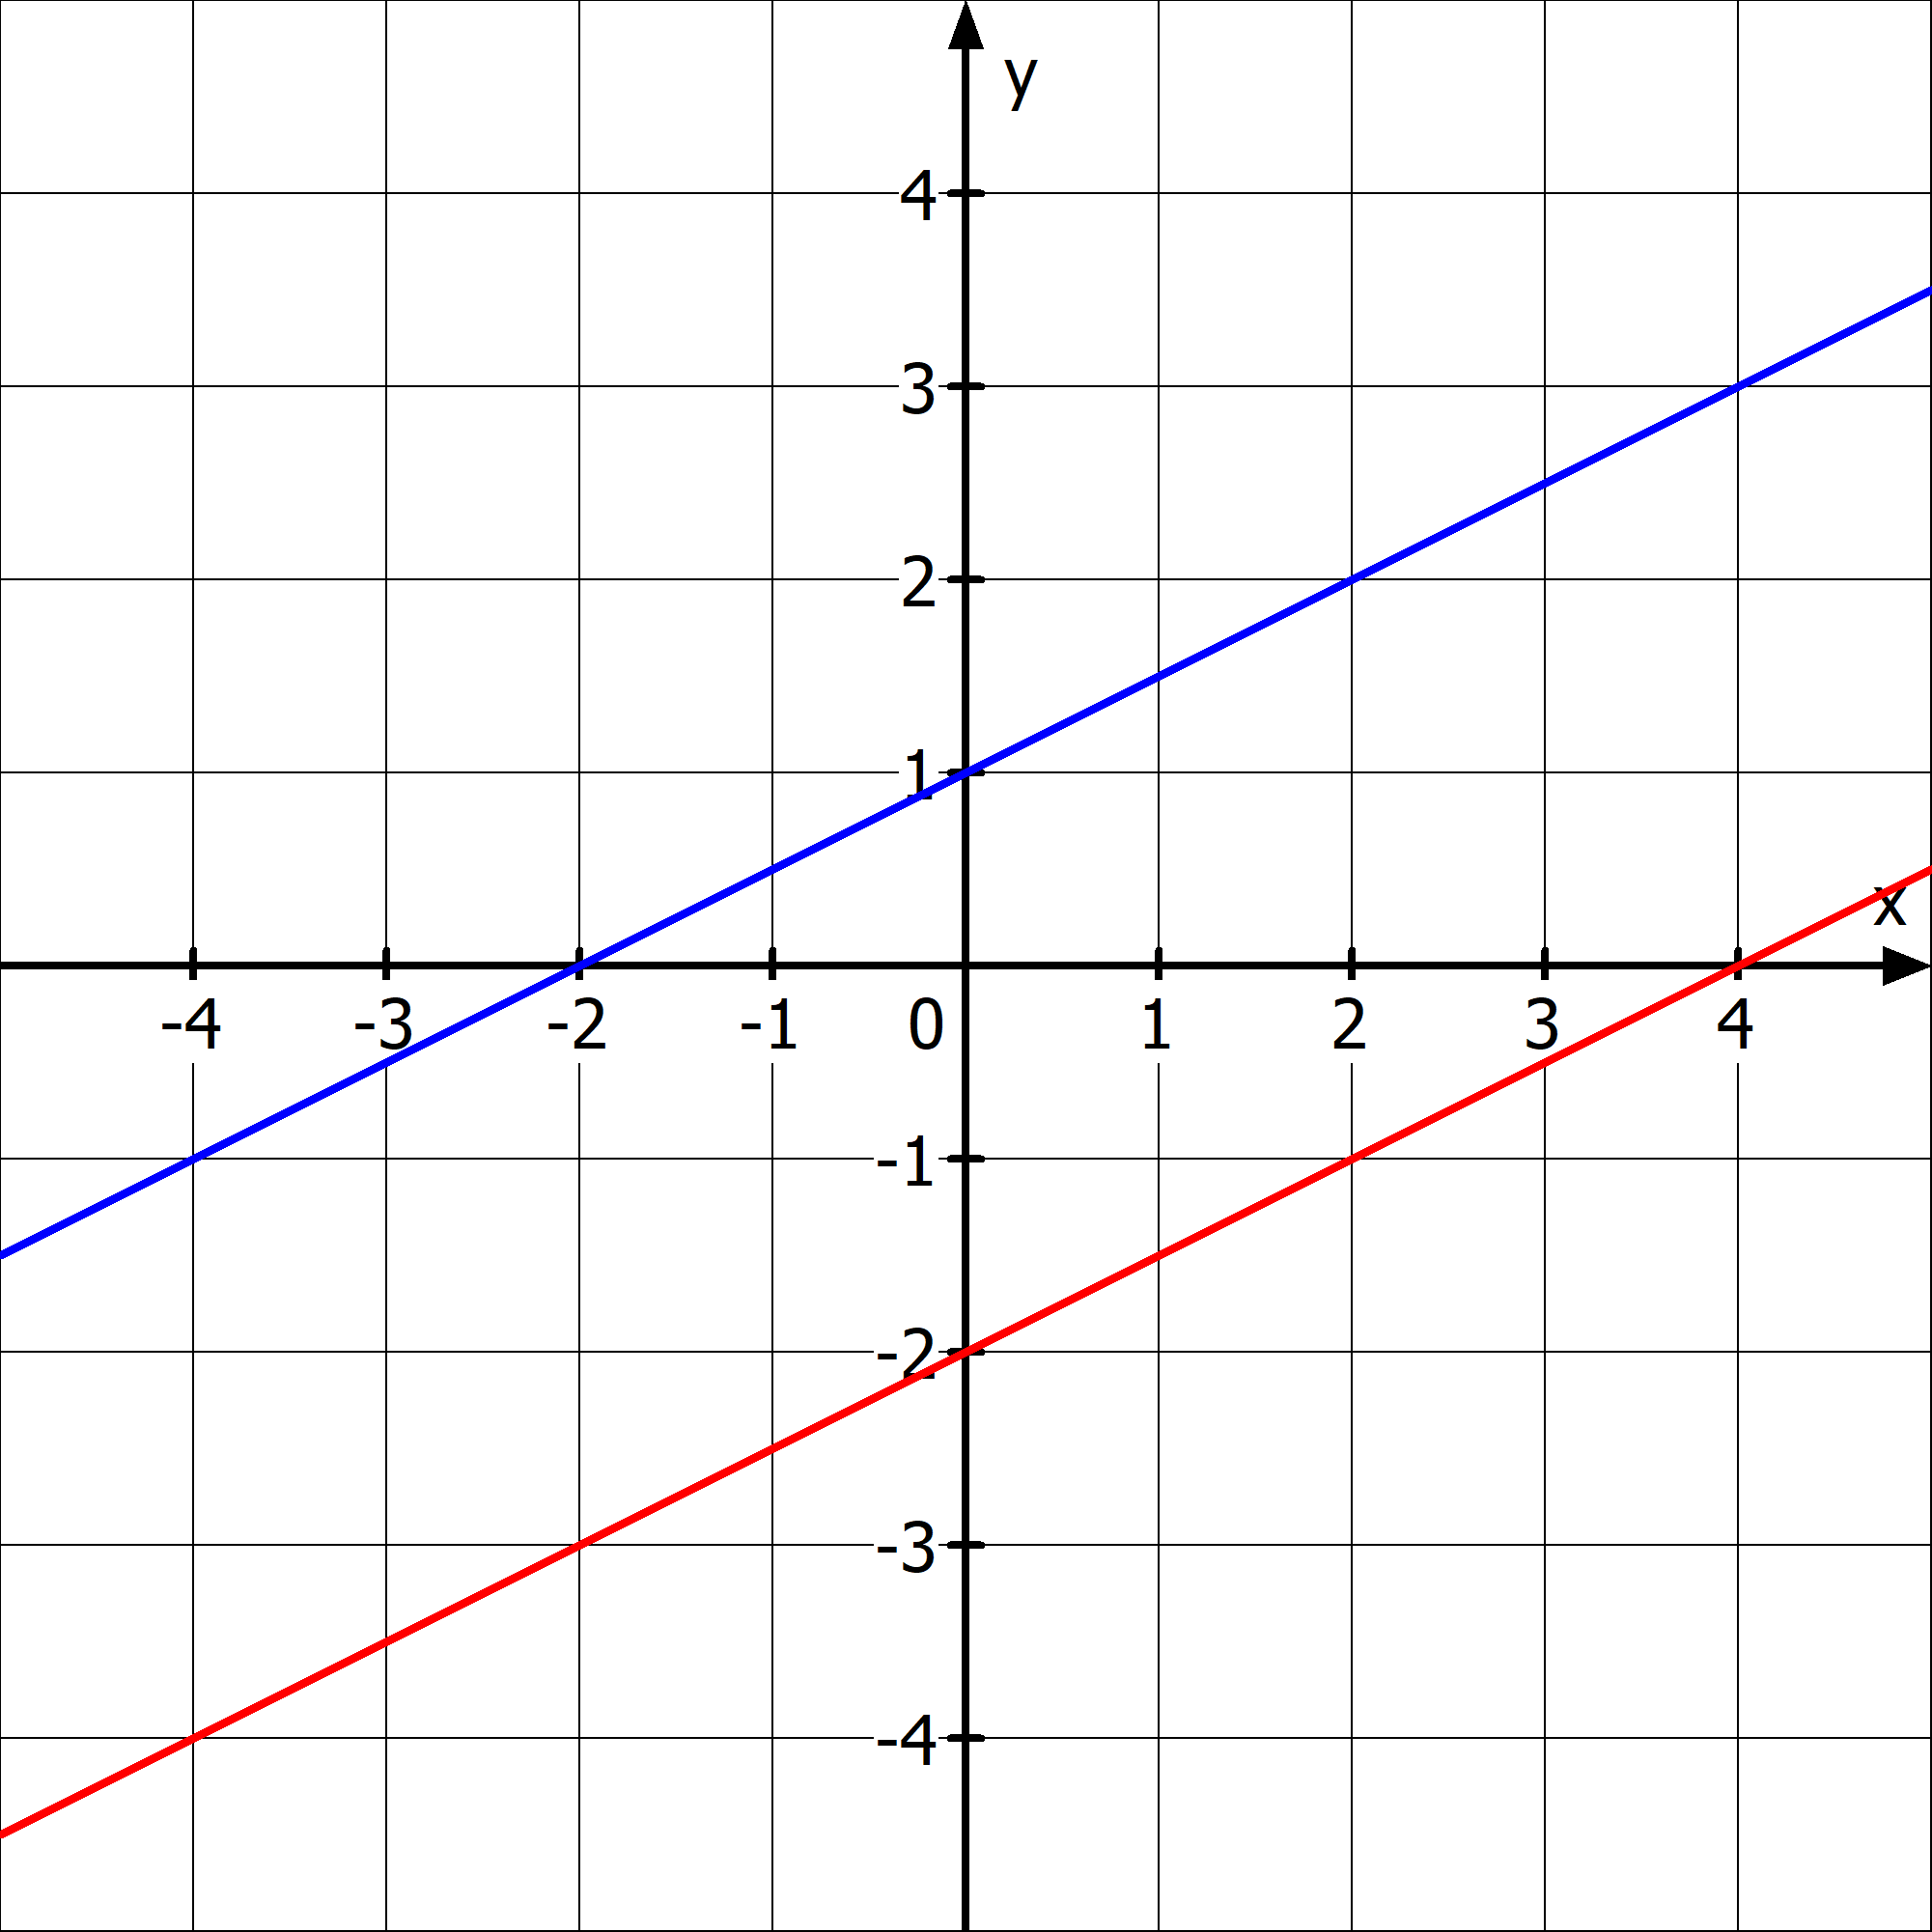
\includegraphics[width=0.45\textwidth]{\linFkt/pics/lage1.png} &
	\parbox[b]{0.46\textwidth}{\raggedright
		\begin{tcolorbox}\centering
			\textcolor{loestc}{$m_f=m_g$}
		\end{tcolorbox}
		\textcolor{loes}{Die beiden Geraden haben die gleiche Steigung. Solche Paare von Geraden nennt man parallele Geraden. Sie haben keinen Schnittpunkt, d.h. die Gleichung $f(x)=g(x)$ hat keine Lösungen. Paralle Geraden, die auch den gleichen y-Achsenabschnitt haben, nennt man identische Geraden. In diesem Fall ist jedes $x$ eine Lösung der Gleichung $f(x)=g(x)$}.\vspace{1cm}
	}
	\\
	$f_1(x)=\tfrac{1}{2}x-2\qquad g_1(x)=0,5x+1$ & \\
	\midrule
	{\Large\textcolor{loes}{keine besondere Lage}} & {\Large\textcolor{loes}{Senkrechte Geraden}}\\
	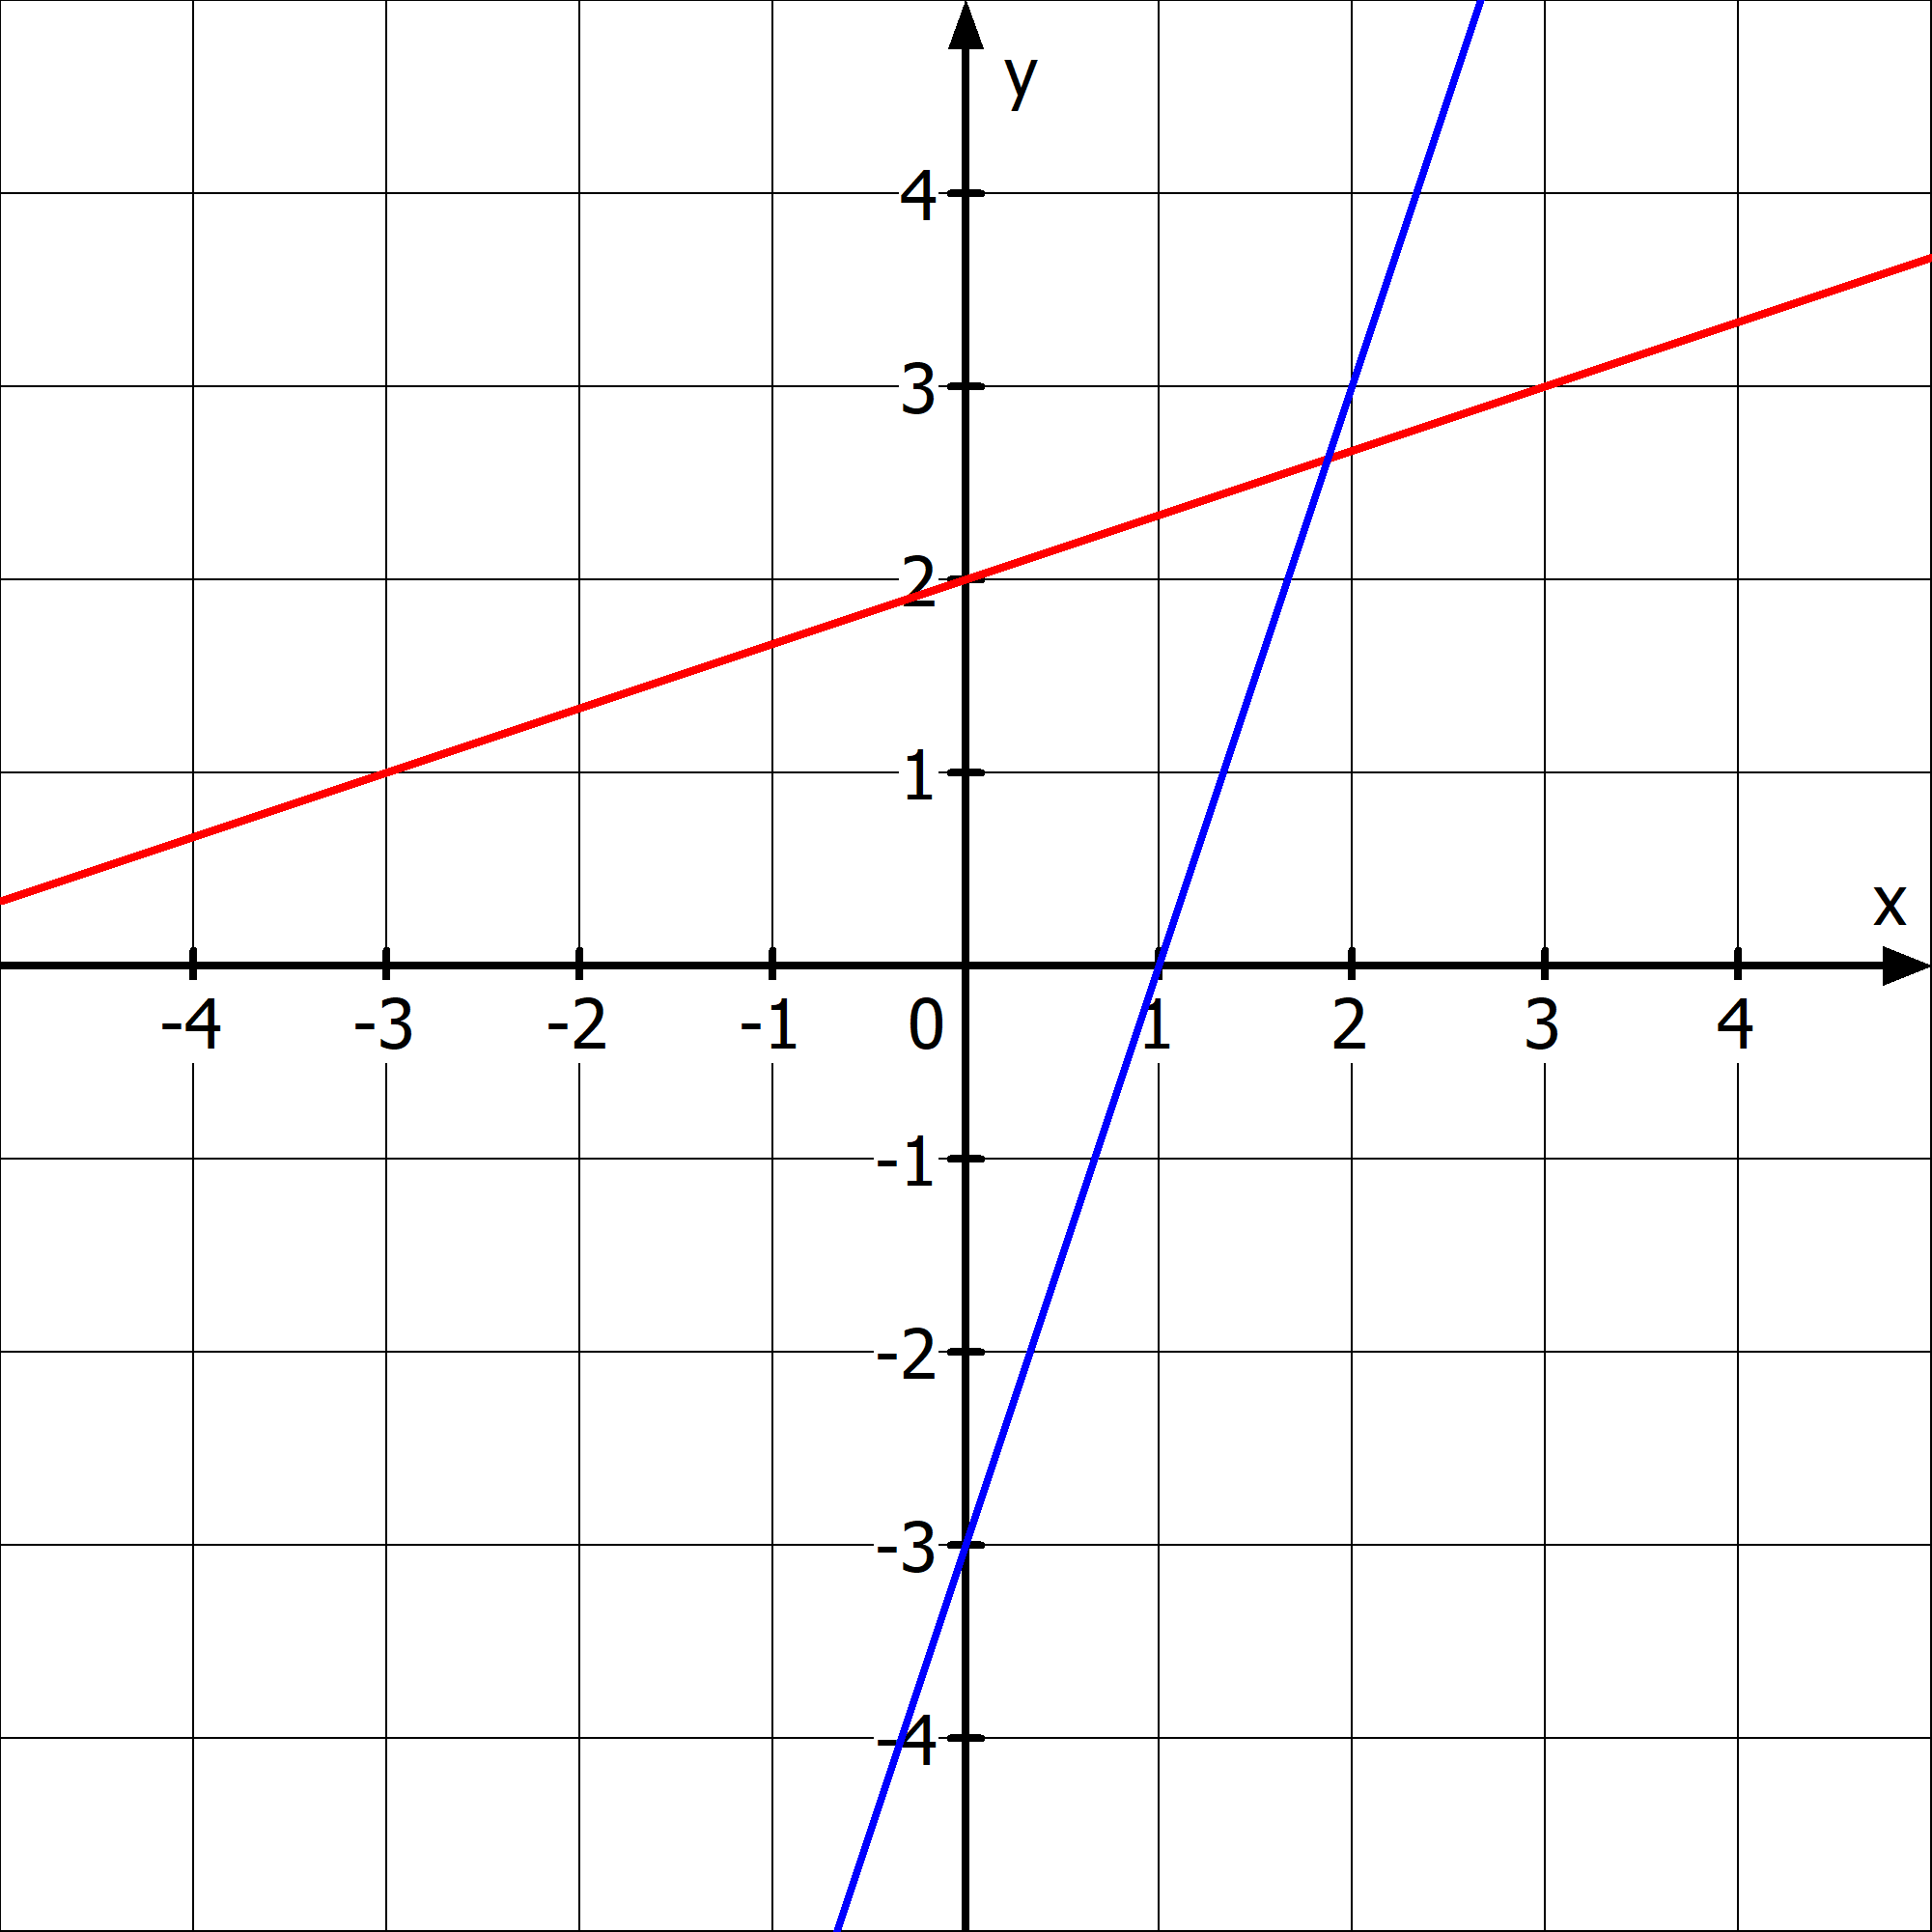
\includegraphics[width=0.5\textwidth]{\linFkt/pics/lage3.png} &
	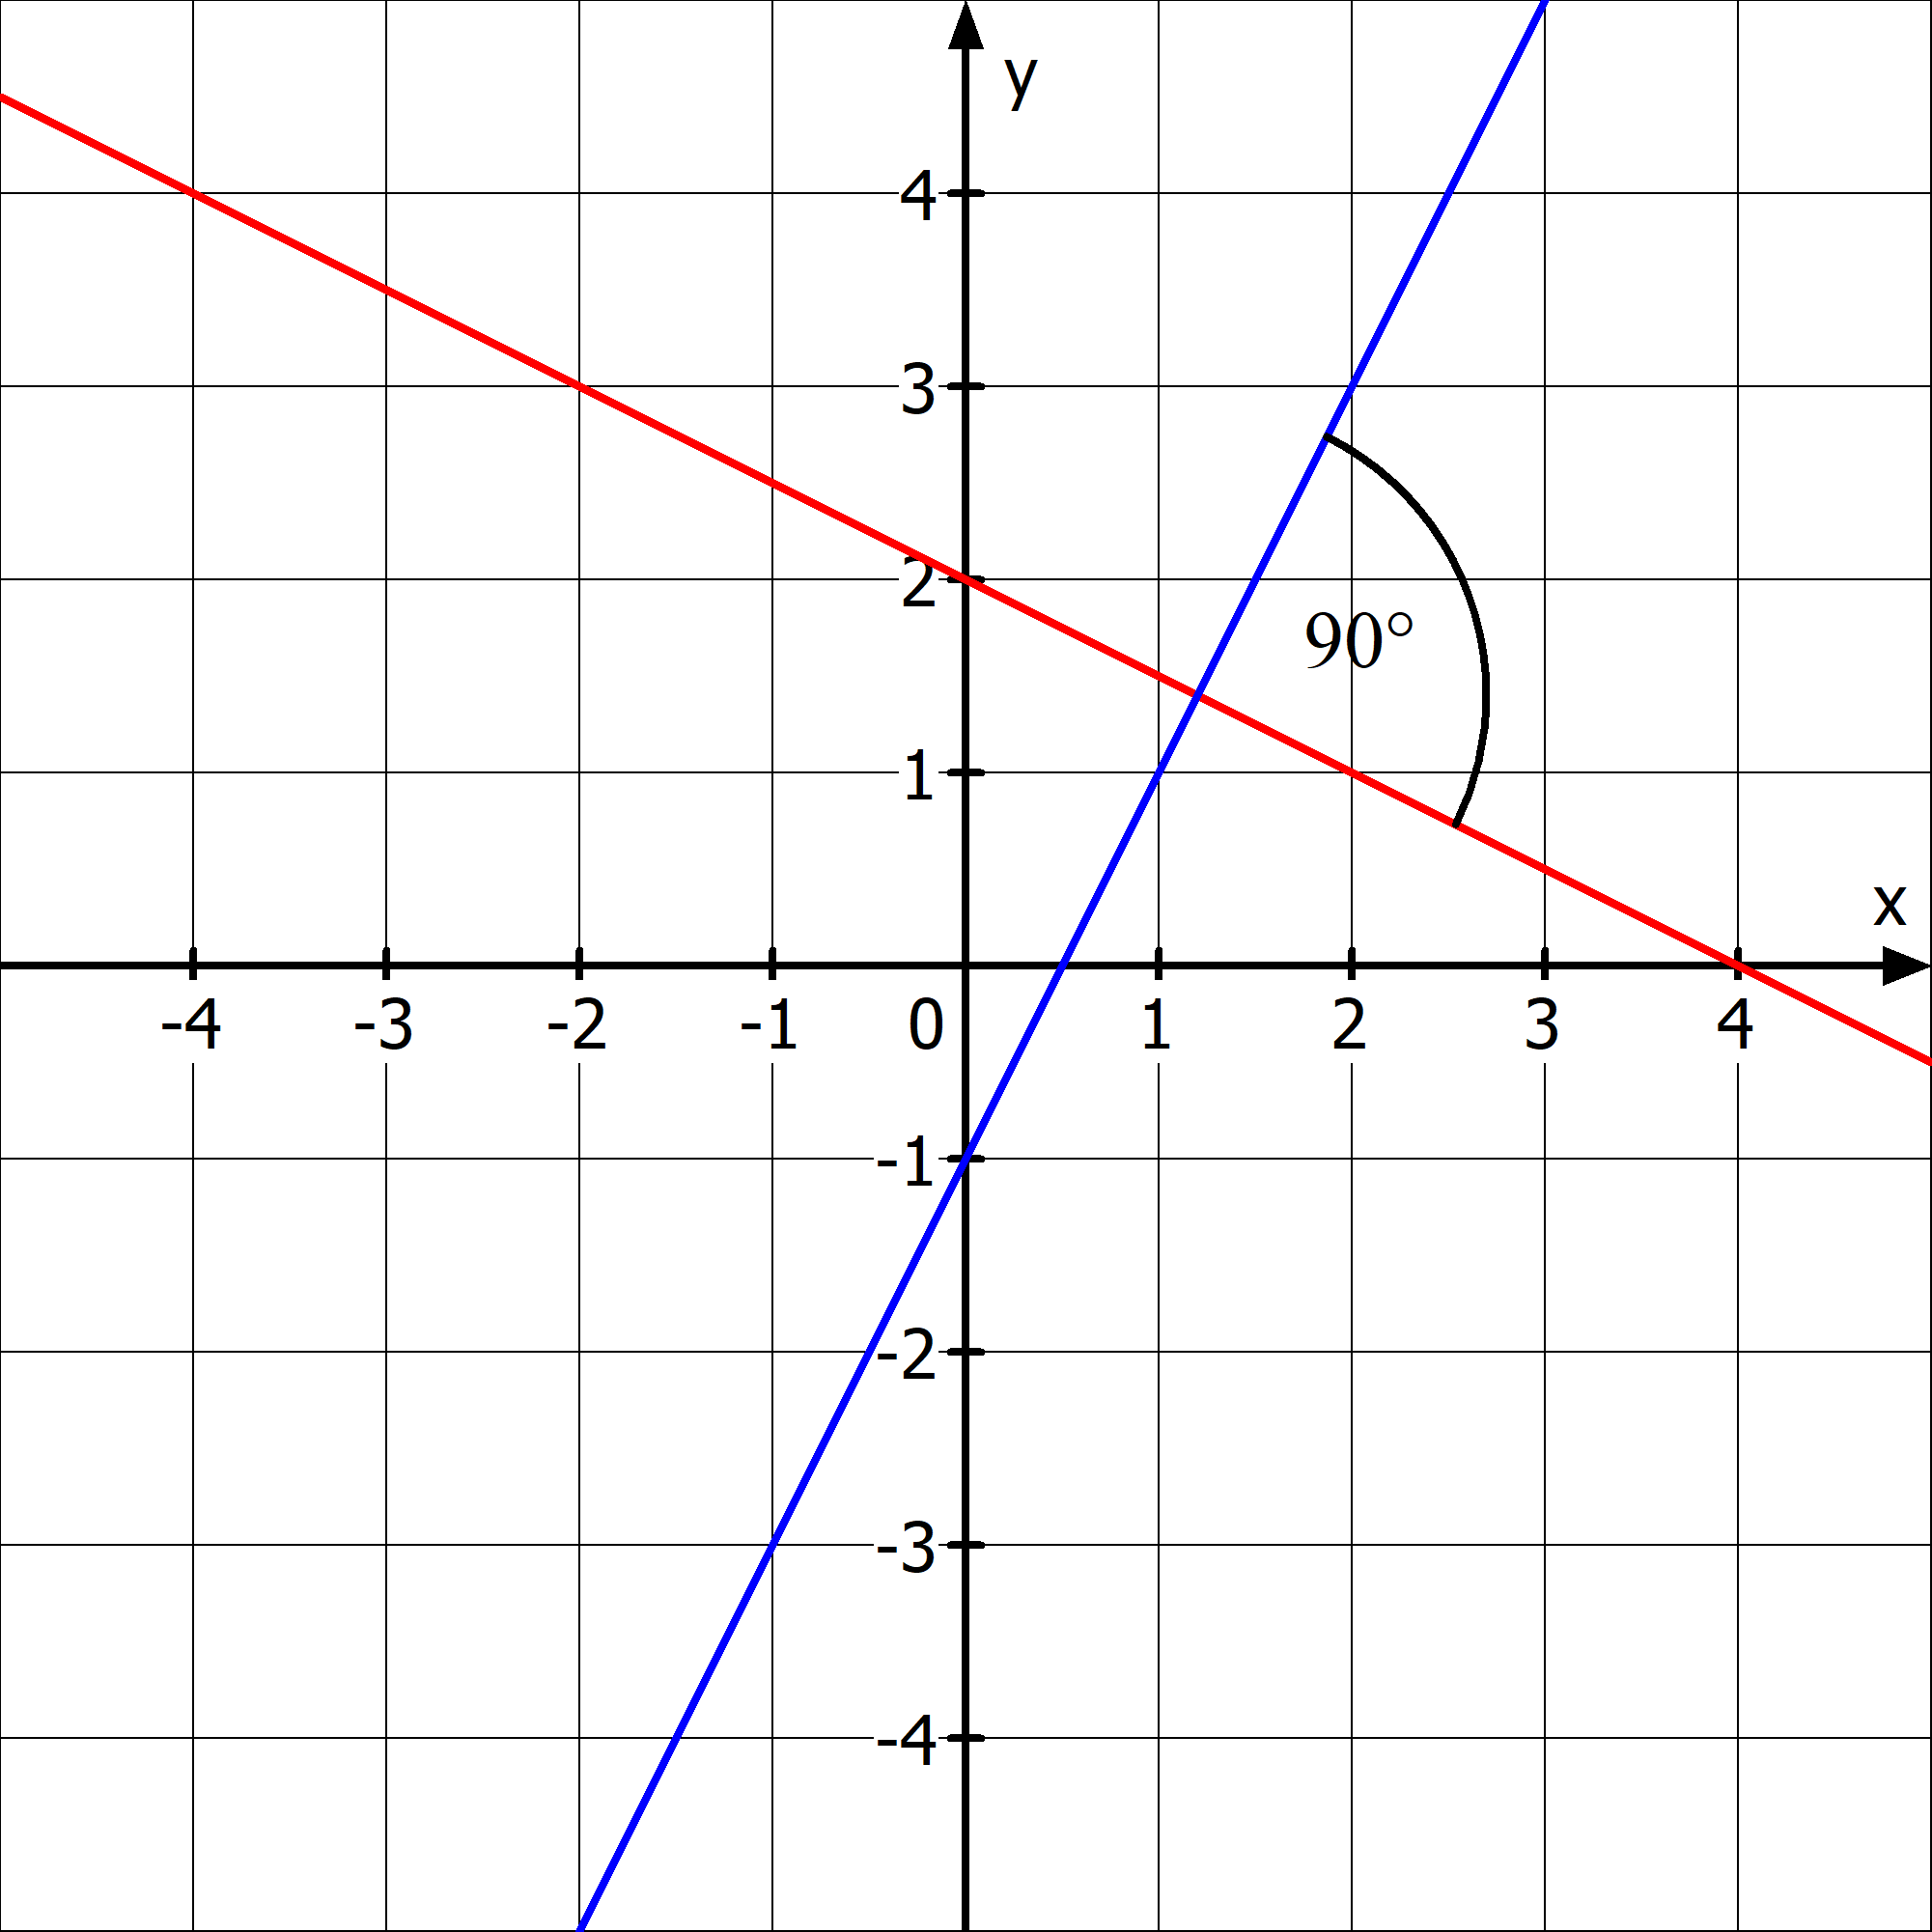
\includegraphics[width=0.5\textwidth]{\linFkt/pics/lage2.png}\\
	$f_3(x)=\tfrac{1}{3}x+2\qquad g_3(x)=3x-3$ &
	$f_2(x)=-\tfrac{1}{2}x+2\qquad g_2(x)=2x-1$\\
	\parbox[t][][t]{0.46\textwidth}{\raggedright
	\begin{tcolorbox}\centering
		\textcolor{loestc}{$m_f\neq m_g$ und $m_f\cdot m_g\neq-1$}
	\end{tcolorbox}
	\textcolor{loes}{Die beiden Geraden sind weder parallel noch orthogonal, d.h. sie haben keine besondere Lage zueinander.}.}&
	\parbox[t][][t]{0.46\textwidth}{\raggedright
	\begin{tcolorbox}\centering
		\textcolor{loestc}{$m_f\cdot m_g=-1$}
	\end{tcolorbox}
	\textcolor{loes}{Die beiden Geraden schneiden sich in einem rechten Winkel. Solche Paare von Geraden stehen orthogonal bzw. normal zueinander.
	}}\\
\end{tabular}